\documentclass[conf]{new-aiaa}
%\documentclass[journal]{new-aiaa} for journal papers
\usepackage[utf8]{inputenc}

\usepackage{graphicx}
\usepackage{amsmath}
\usepackage[version=4]{mhchem}
\usepackage{listings}
\usepackage{color}
\usepackage{siunitx}
\usepackage{longtable,tabularx}
\usepackage{subcaption}
\usepackage{cleveref}
\usepackage{appendix}
\setlength\LTleft{0pt}

\title{AE625 - Computational Fluid Dynamics \\ Assignment - 05 \\ Numerical simulation of Lid Driven Cavity Flow Problem}

\author{Ramkumar S. \footnote{SC22M007, M.Tech., Aerospace AFM }}
\affil{SC22M007, M.Tech. Aerospace - Aerodynamics and Flight Mechanics}


\definecolor{mygreen}{rgb}{0,0.6,0}
\definecolor{mygray}{rgb}{0.5,0.5,0.5}
\definecolor{mymauve}{rgb}{0.58,0,0.82}

\lstset{
  backgroundcolor=\color{white},   % choose the background color; you must add \usepackage{color} or \usepackage{xcolor}; should come as last argument
  basicstyle=\footnotesize,        % the size of the fonts that are used for the code
  breakatwhitespace=false,         % sets if automatic breaks should only happen at whitespace
  breaklines=true,                 % sets automatic line breaking
  captionpos=b,                    % sets the caption-position to bottom
  commentstyle=\color{mygreen},    % comment style
  deletekeywords={...},            % if you want to delete keywords from the given language
  escapeinside={\%*}{*)},          % if you want to add LaTeX within your code
  extendedchars=true,              % lets you use non-ASCII characters; for 8-bits encodings only, does not work with UTF-8
  firstnumber=0001,                % start line enumeration with line 1000
  frame=single,                    % adds a frame around the code
  keepspaces=true,                 % keeps spaces in text, useful for keeping indentation of code (possibly needs columns=flexible)
  keywordstyle=\color{blue},       % keyword style
  language=Octave,                 % the language of the code
  morekeywords={*,...},            % if you want to add more keywords to the set
  numbers=left,                    % where to put the line-numbers; possible values are (none, left, right)
  numbersep=5pt,                   % how far the line-numbers are from the code
  numberstyle=\tiny\color{mygray}, % the style that is used for the line-numbers
  rulecolor=\color{black},         % if not set, the frame-color may be changed on line-breaks within not-black text (e.g. comments (green here))
  showspaces=false,                % show spaces everywhere adding particular underscores; it overrides 'showstringspaces'
  showstringspaces=false,          % underline spaces within strings only
  showtabs=false,                  % show tabs within strings adding particular underscores
  stepnumber=2,                    % the step between two line-numbers. If it's 1, each line will be numbered
  stringstyle=\color{mymauve},     % string literal style
  tabsize=2,                       % sets default tabsize to 2 spaces
  % title=\lstname                 % show the filename of files included with \lstinputlisting; also try caption instead of title
}

\begin{document}

\maketitle

\begin{abstract}
    The numerical computation of 2D lid driven cavity flow problem was performed
    with the domain of size 2X2 meters with top wall being moved at 1m/s velocity.
    Air is chosen as the working fluid with incompressibility assumption. The
    simulation was performed using finite difference method on a staggered grid
    using pressure correction technique and SIMPLE algorithm. Solutions obtained
    were post-processed for a range of timesteps and the contours of pressure,
    velocity magnitude and voricity were made. the streamlines were also
    plotted and the animations showing the change in flow field were also
    generated.
\end{abstract}


%------------------------------------------------------------------------------
\begin{frame}
    \frametitle{Problem Definition}
    2D square plate of side 1 m with one hot side and other 3 cold sides
    \begin{figure}
        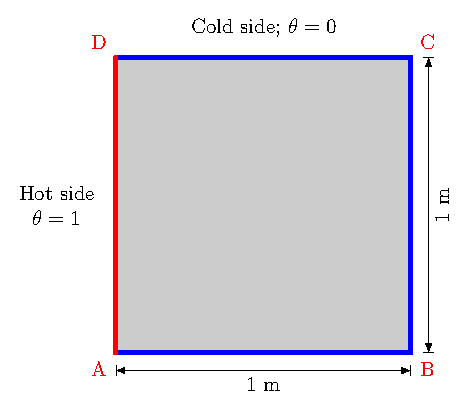
\includegraphics[scale=0.7]{00_schematic/01_problem_schematic/problemDefinition.pdf}
    \end{figure}

    Present work is to compute the temperature field within plate domain
    using PINNs with different variations in methodology.
\end{frame}

%------------------------------------------------------------------------------
\begin{frame}
    \frametitle{Governing equation and Analytical solution}

    \begin{figure}
        \centering
        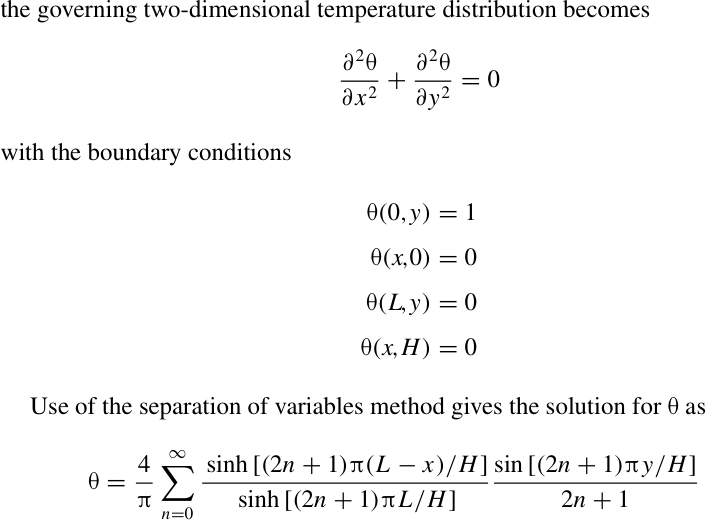
\includegraphics[scale=0.4]{supportingFiles/eqn.png}
    \end{figure}
\end{frame}

%------------------------------------------------------------------------------

\begin{frame}
    \frametitle{Network Schematic}
    \begin{figure}
        \centering
        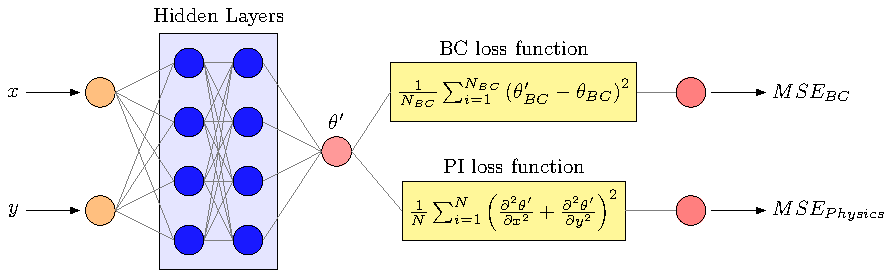
\includegraphics[scale=0.77]{00_schematic/02_PINN_schematic/PINN_HC_schematic.pdf}
    \end{figure}
\end{frame}

%------------------------------------------------------------------------------

\begin{frame}
    \frametitle{key points}

    \begin{itemize}
        \item pure physics-based training was done on the network with 20NX8L size,
            with 40 boundary points and 100 internal points.
            \vspace{1cm}
        \item the model was trained with 40,000 epochs and took about 3 minutes.
            Then the model is used to predict the solution on a 1 million grid.
            \vspace{1cm}
        \item The grid-extended solution was compared with analytical solution,
            the numerical solution was attempted for the same grid using FDM on
            FORTRAN with Gauss-seidel method.
    \end{itemize}
\end{frame}

%------------------------------------------------------------------------------

\begin{frame}
    \frametitle{Run-time comparison: PINN vs FDM}
    On 1 million grid,
    \begin{itemize}
        \item PINN took 172.42 seconds (2.87 minutes), including training time
        \item FDM took 1635.79 seconds (27.63 minutes)
    \end{itemize}
    \begin{columns}

        \begin{column}{0.5\textwidth}
            \begin{figure}
                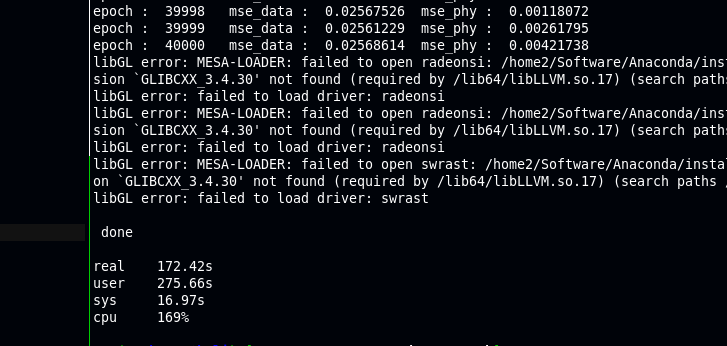
\includegraphics[scale=0.3]{supportingFiles/runtime_PINN.png}
                \caption{PINN runtime}
            \end{figure}
        \end{column}

        \begin{column}{0.5\textwidth}
            \begin{figure}
                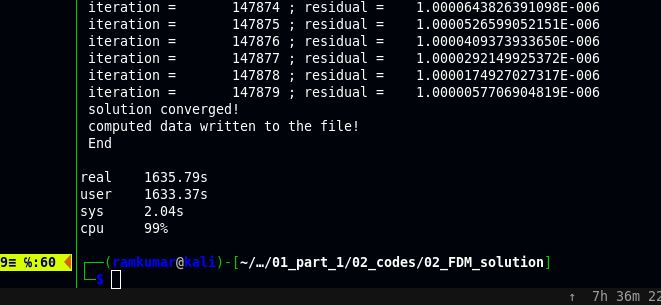
\includegraphics[scale=0.3]{supportingFiles/runtime_FDM.png}
                \caption{PINN runtime}
            \end{figure}
        \end{column}

    \end{columns}
\end{frame}

%------------------------------------------------------------------------------

\begin{frame}
    \frametitle{Solution Comparison: PINN vs Analytical : 1 Mil grid}
    \begin{figure}
        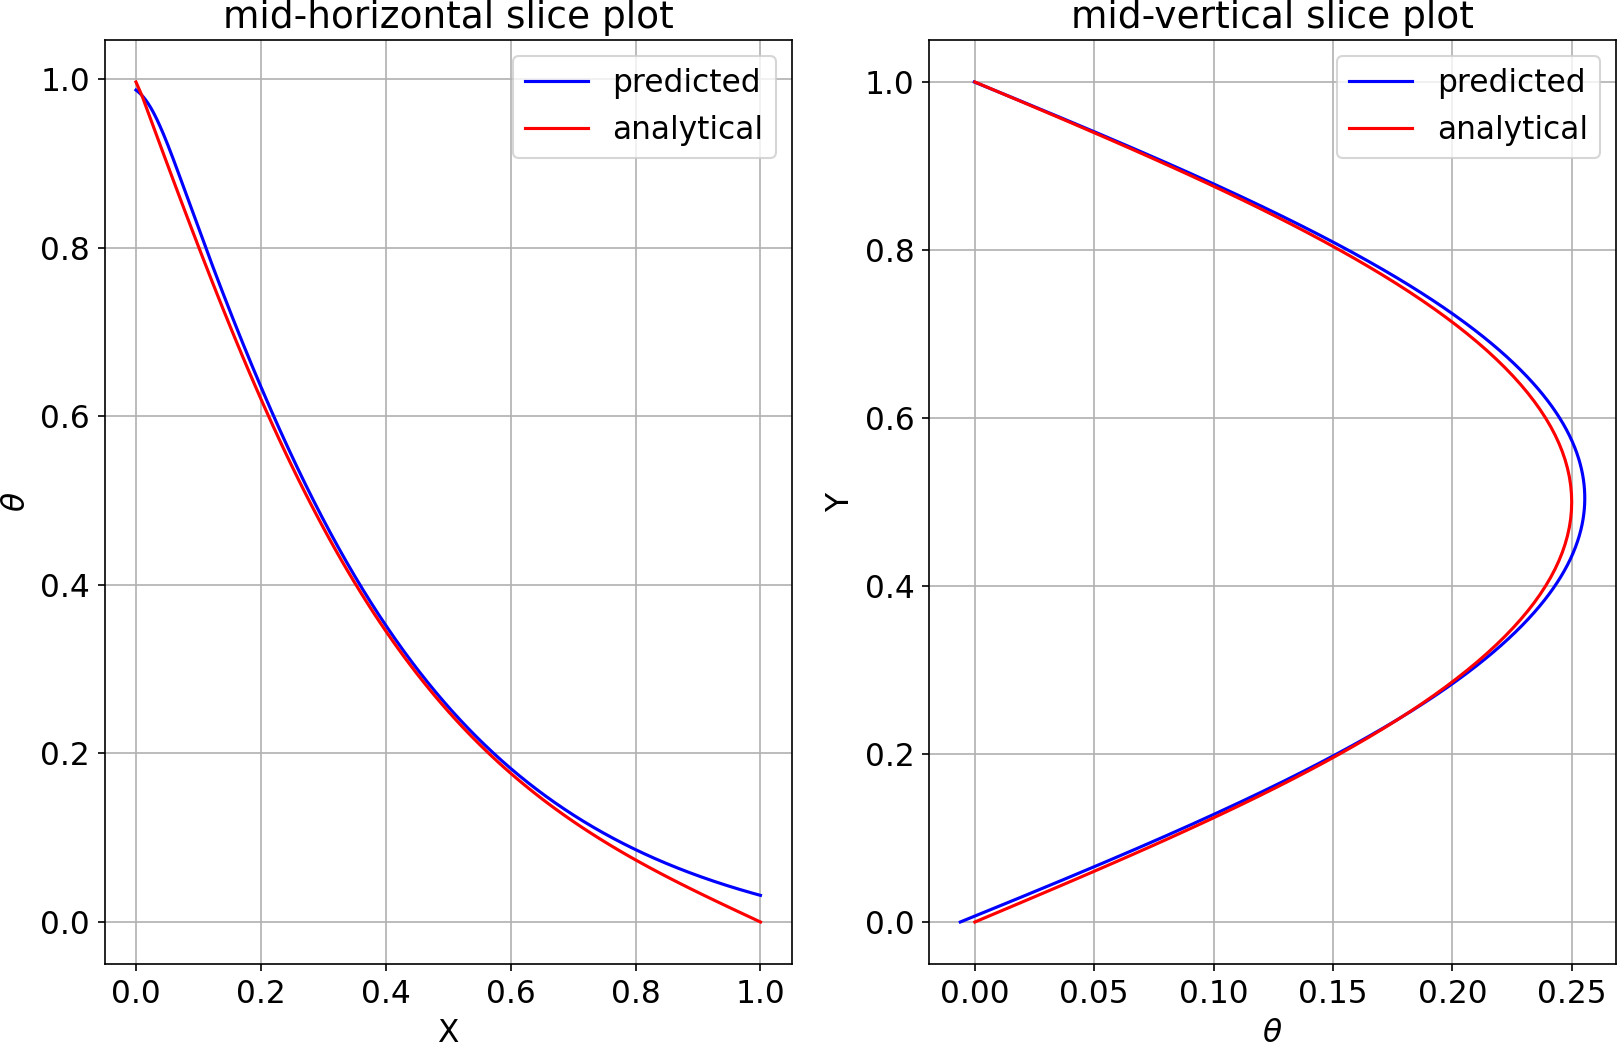
\includegraphics[scale=0.4]{supportingFiles/slice_plots_out.png}
    \end{figure}
\end{frame}

\begin{frame}
    \frametitle{Solution Comparison: PINN vs Analytical : 1 Mil grid}
    \begin{figure}
        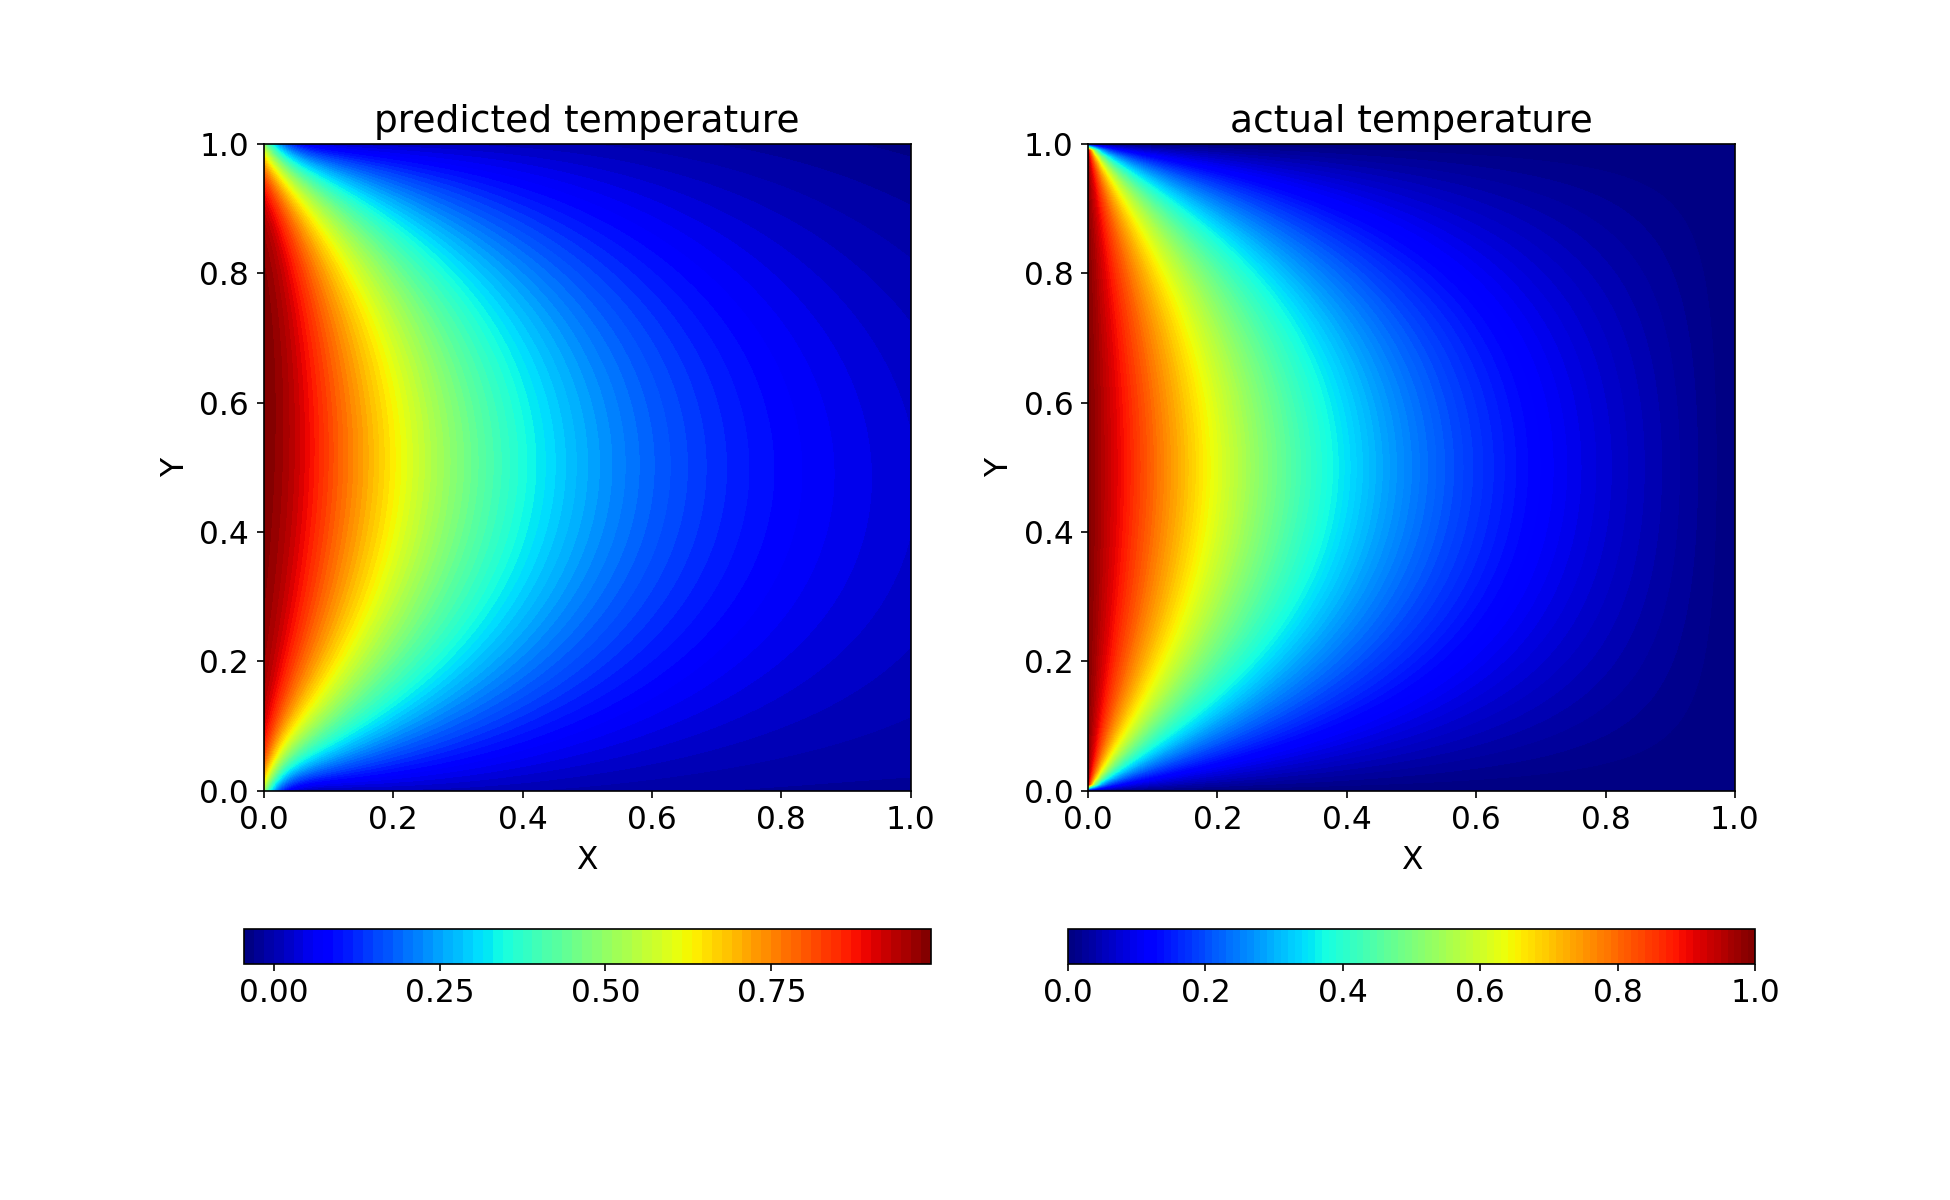
\includegraphics[scale=0.4]{supportingFiles/contours_out.png}
    \end{figure}
\end{frame}

%------------------------------------------------------------------------------

\begin{frame}
    \frametitle{Solution Comparison: FDM vs Analytical : 1 Mil grid}
    \begin{figure}
        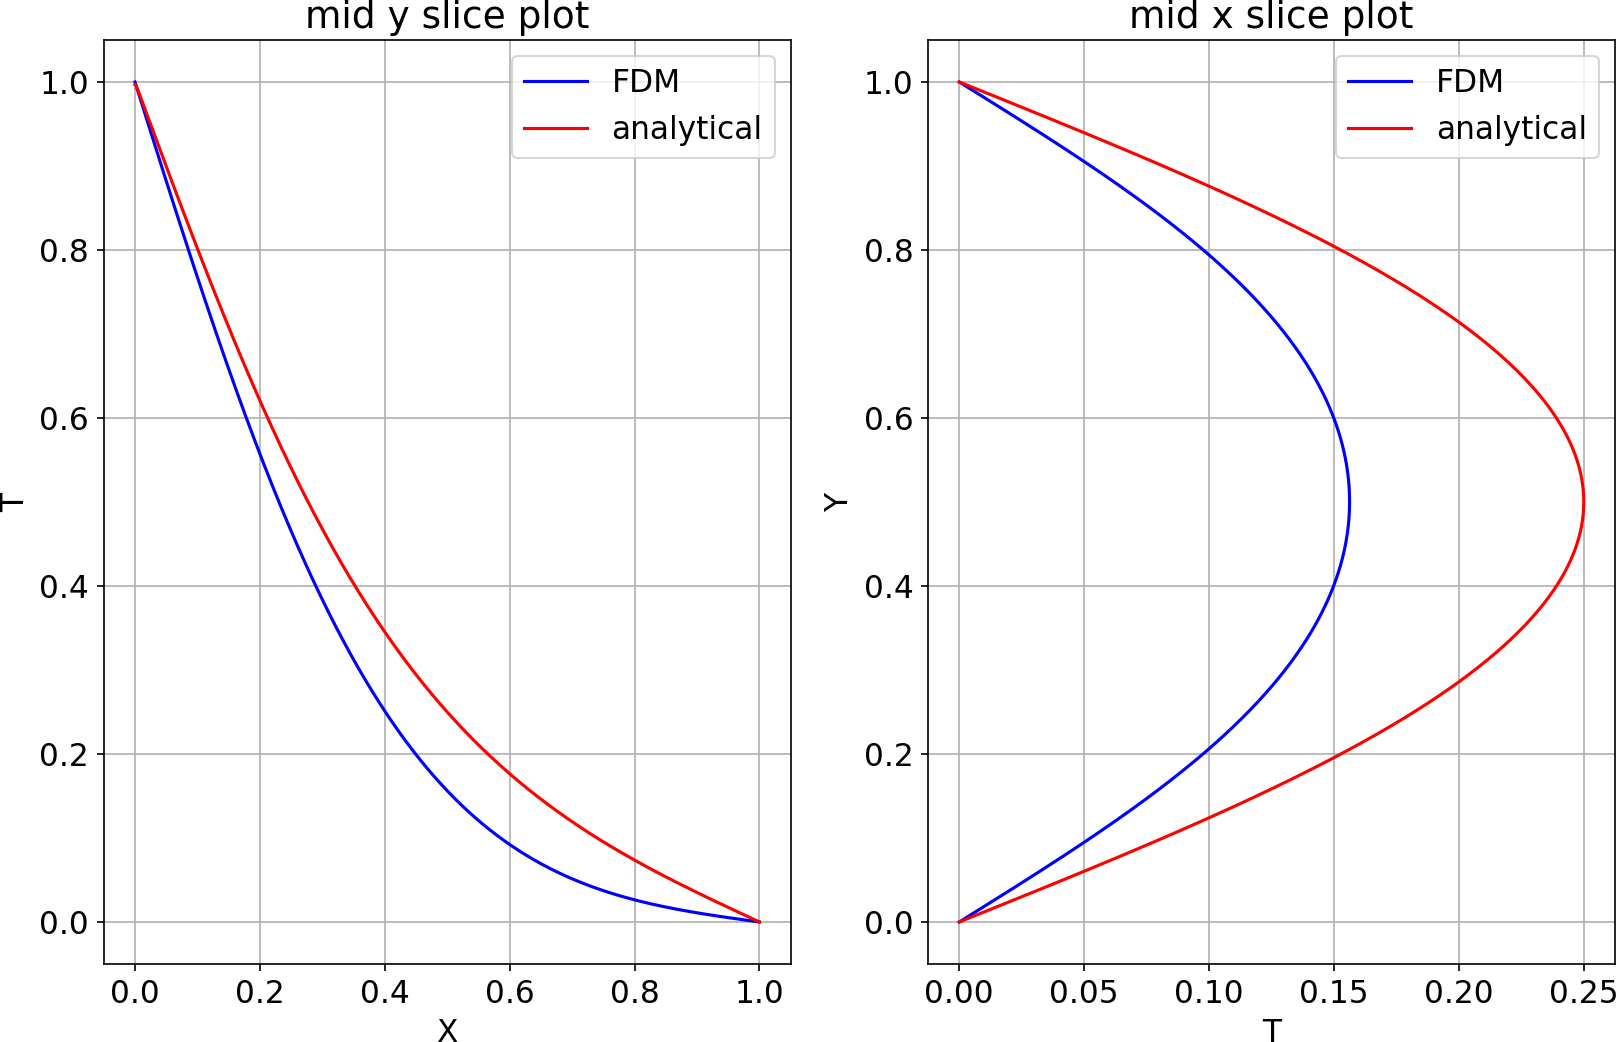
\includegraphics[scale=0.4]{supportingFiles/plots_FDM.png}
    \end{figure}
\end{frame}

%------------------------------------------------------------------------------

\begin{frame}
    \frametitle{Conclusion}
    \begin{enumerate}
        \item FDM solution did not match with analytical solution despite its
            convergence.
            \vspace{0.5cm}
        \item PINN's grid-extended solution matches with analytical solution.
            \vspace{0.5cm}
        \item PINN learns the function quite well by solving the problem with
            just 140 data points in the domain.
            \vspace{0.5cm}
        \item The time taken by PINN is 10 times less than FDM for the same
            grid solution, including training time.
            \vspace{0.5cm}
        \item PINN solution can be used as initial condition for steady state
            problems on large grids to save computational time.
    \end{enumerate}
\end{frame}


\begin{thebibliography}{2}
    \bibitem{ref_1} McLay, A. "Computational Fluid Dynamics: the Basics with Applications, JD Anderson, McGraw-Hill Book Company Europe, McGraw-Hill House, Shoppenhangers Road, Maidenhead, Berkshire SL6 2QL. 1995. 547pp. Illustrated.£ 23.95." The Aeronautical Journal 100.998 (1996): 365-365.
\end{thebibliography}

\pagebreak

\begin{appendices}

    \section{Appendix - FORTRAN and Python codes}\label{numerical_code}
    This section contains the FORTRAN and Python source codes used in solving
    the lid driven cavity flow problem.

    \par Main solver FORTRAN code
    \lstinputlisting[language=Fortran]{supporting_documents/main.f08}

    \par Parameters module FORTRAN code
    \lstinputlisting[language=Fortran]{supporting_documents/parameters.f08}

    \par Subroutines Module FORTRAN code
    \lstinputlisting[language=Fortran]{supporting_documents/subroutines.f08}

    \par The Python script for postProcessing the data
    \lstinputlisting[language=Python]{supporting_documents/script_plotter.py}

\end{appendices}

\par
\center{**********}

\end{document}
